\chapter{Section Two} \label{cha:litrev}
\section{Literature Review}
\subsection{Android Permission Model}
\subsubsection{Comparison of Application Approval Process}

The leading mobile operating systems apart from Android are iOS by Apple, Windows Mobile and BlackBerry OS. Each of these have different processes and methodologies for developers to follow before submitting an application to the store. A comparison between application submission processes for these platforms shows that each has a centralized process for validation and/or verifying an application before it is made available for users to download. However these processes are usually in place for checking security or applications, and not privacy related issues. 
\smallskip

To submit an application to iTunes, the marketplace for iOS applications, the developer is first required to create an App ID and a Distribution Provisioning Profile and then  submit an application through iTunes connect with detailed information on the app.Three different certificates have to be submitted along with the application; the Distribution Certificate, Push Notification Certificate and Mobile Provisioning Certificate. The app has to be submitted through the Publication Center, where a checklist of complying standards that need to be adhered to has to be filled in.The approval process on average takes six days to one week.\cite{e}
\smallskip

Windows store applications also go through a centralized process before being released. A submission has to be created for each application with a checklist of information. Once the submission is complete and the application has been preprocessed without errors, it is submitted for certification through the Windows Certification Kit. The certification process focuses on three core areas; security tests, technical compliance tests and content compliance tests. The amount of time taken for an application to receive approval fluctuates based factors such as the code and logic complexity, visual content, rating of the developer, other applications in the queue etc. Applications which fail the certification process will be returned with a report indicating where the compliance standards were not met. Developers are allowed to resubmit applications following the same process.\cite{f}
\smallskip

RIM(Research In Motion) BlackBerry requires developers to submit applications for a complex process of reviewing, testing and "readying for publication" before being awarded a Approved/Up For Sale rating. Apps with this rating can be submitted and released on the BlackBerry marketplace; BlackBerry App World.\cite{j} 
\smallskip

Android developers add applications to marketplaces including Google PlayStore, Amazon AppStore, GetJar, SlideMe and F-Droid, which can then be downloaded by users. The problem lies in there being no centralized security measurement for applications on such marketplaces. Developers are trusted to prepare an application for release and then release it through a marketplace, email or website.\cite{g} The Android operating system imposes some security and privacy restrictions, including an install-time permission system, where each application declares what permissions it requires upon installation.\cite{h} This can provide users with control over their privacy since the choice to cancel installation lies with the user.

\subsubsection{Application Security and Privacy}
The Android OS is built on top of the Linux kernel, which manages the hardware including drivers and power management. From the bottom-up, the next layers include HAL or the Hardware Abstraction Layer, Native libraries and the runtime, which includes the Dalvik virtual machine, the framework with activity managers, system view and content providers, and a layer of applications(Refer Figure 2.1). Each time a new application is installed, the operating system assigns it a unique Linux user ID, which will be persistent for the lifetime of the application on that device. On uninstallation of an application, the user ID will be freed and possibly reassigned to another new application after the device is rebooted for the first time following an uninstallation.
\smallskip 

Permissions are tied to the user IDs, attemting to provide application sandboxing and process isolation by limiting communication between applications to methods overseen by the operating system such as passing of intents. Applications get a dedicated part of the file system connected to its UID whiich can be used to write private data and store databases and raw files, including permission information. According to the description on the Android Security website, the OS "seeks to be the most secure and usable operating system for mobile platforms by re-purposing traditional operating system security controls to protect user data, protext sstem resources and provide application isolation by providing robust security at the OS level through the Linux kernel, mandatory application sandbox for all applications, secure interprocess communication, application signing and application-defined and user-granted permissions"\cite{diagrameka}. However, this system has several loopholes, and malicious applications can access sensitive resources even in cases where sandboxing is done by the user ID system\cite{meshram2014survey}. 
\smallskip
\begin{figure}
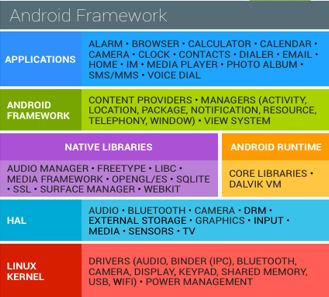
\includegraphics[totalheight=6cm]{Capture1}
\caption{The Android Software Stack}
\end{figure}
\smallskip

\subsubsection{Installing Applications}
The Android OS allows users to install both free and paid third party Java applications through markets such as Google Play. As discussed Android applications do not go through a review process to measure compliance to guidelines, although most competitors including iOS, Windows and RIM do. Access to sensitive resources, also known as "permissions" are controlled by the operating system to let aplications request access to sysytem functionality through an XML manifest, forming a computer-supported-access-system(CSAS)\cite{stevens2009computer}. Applications are allowed to define their own extra permissions in addition to the 134 core permissions provided by Android\cite{a}. (This research will not focus on third party defined permissions.)
\smallskip

Google Play application listings show information about each application including screenshots, marketing jargon, compatibility with user devices, app information, developer information, content rating, reviews and other related applications. However this does not include a list of permissions used by the app, or any privacy or security related information on the application page. Once a user clicks on the install button, they are expected to approve or disapprove the permission list that appears when downloading on devices older than Android M, without any background information. Permissions and privacy information are not highlighted on both the mobile application of Google Play or the store website\cite{kelley2013privacy}. 

\subsubsection{Before Android Marshmallow}
Before Android sdk 23, the permission model was based on a "do-or-die" concept. Users were given a list of permissions that would be required upon clicking the "install" link on an application on Google Play. There were no options to grant permissions selectively or revoke when not needed, and choosing not to grant a particular permission resulted in the application installation process being terminated\cite{felt2011effectiveness}. User choice was limited to whether they wanted to use the application, or not, and this has caused habituation even in later versions where permissions can be toggled\cite{wijesekera2015android}, since users choose to approve permissions by reflex as part of the installation process of an application. Research has shown that 83\% of application installations happen without the user consciously reading the permission list\cite{felt2012android}. Android Marshmallow is only being run on 10.1\% of all Android devices according the most current dashboard data at the time of writing\cite{androdashboard}, resulting in many users still being forced to follow the do-or-die model when installing applications(refer figure 2.2). 
%, width=0.5\textwidth
\smallskip
\begin{figure}
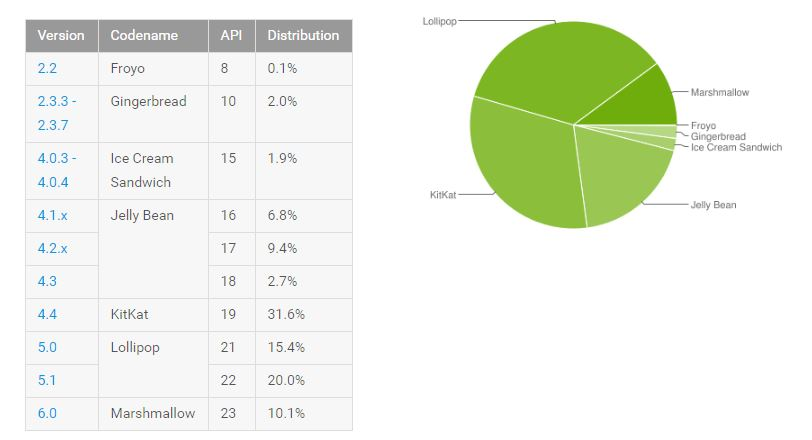
\includegraphics[totalheight=6cm]{Capture2}
\caption{Android Platform Versions as at 30.05.2016\cite{androdashboard}}
\end{figure}
\smallskip

\subsubsection{After Android Marshmallow}
The current permission model assigns permissions into two categories; normal permissions and dangerous permissions(See Appendix 01 for a list of normal and dangerous permissions). Normal permissions are granted automatically when requested by a user, and can alter basic low-risk elements of a device's settings, such as the display brightness or wallpaper. Dangerous permissions are any permissions that can alter sensitive data on the device or use the device's higher-risk functions, such as connecting to the Internet, and are further classified into groups. If a permission from the same group has previously been approved by the user, then the permission will be automatically granted(i.e. if READ\_SMS permission has been approved by the user then the device will not require permission to access the WRITE\_SMS permission either). However, if a dangerous permission is in a category which has not been approved by the user earlier, a popup notification is generated at runtime, asking the user to approve the permission request. The permission, once granted, can be revoked by toggling a control in the application settings page later on. However, it should be noted that there has been criticism of the classification of permissions, and may researchers such as Felt have pointed out in earlier experiments that the classification should be based on risk to user privacy\cite{felt2011android}, resulting in classification systems that do not correlate with what is currently implemented by Google\cite{androidyearinreview}. Refer figure 2.3 for a flowchart highlighting the recommended model for requesting permission in current Android devices.
\smallskip
\begin{figure}
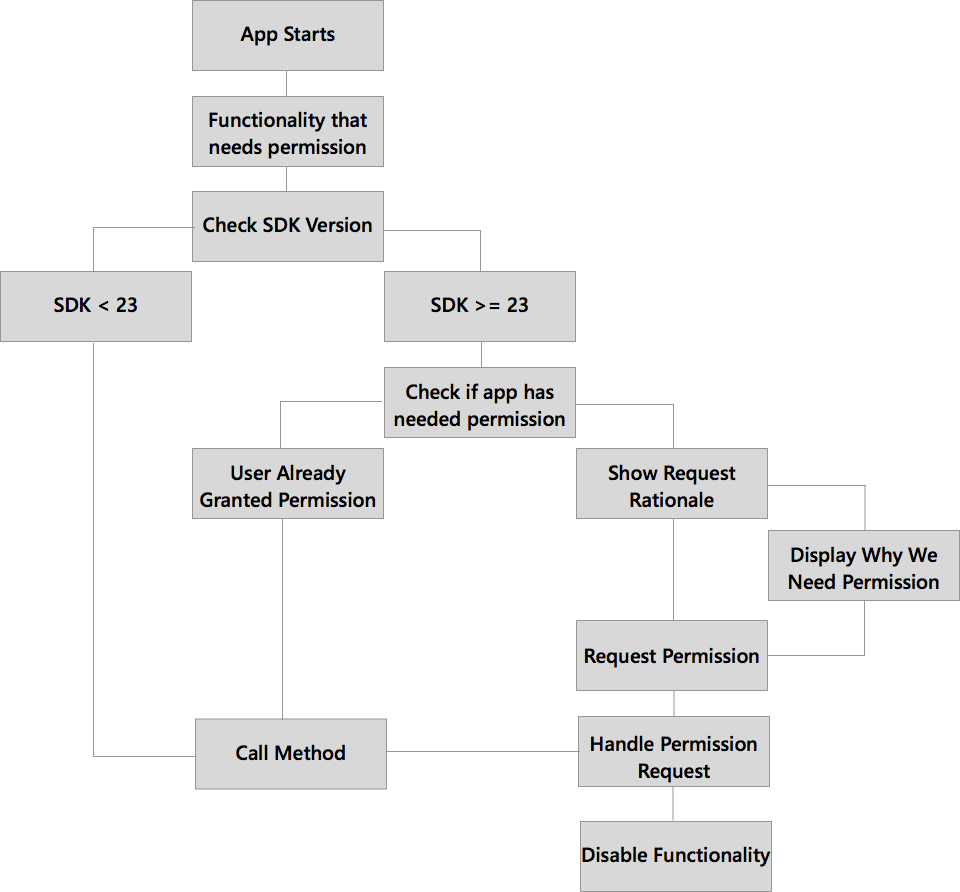
\includegraphics[totalheight=7cm]{Flowchart}
\caption{Android Permission Model- Flowchart\cite{flowchartimage}}
\end{figure}
\smallskip 

\subsection{Problems with the existing system}
The current permission model is problematic and offers loopholes that can be manipulated to compromise privacy of user data. This section will include a condensed view of research in this domain which highlight and offer solutions to some of these issues. 

\subsubsection{Least Privilege}
Both the most popular mobile operating systems, iOS and Android, require that developers follow the principle of "least privilege" with regard to permissions. The principle of least privilege states that "Every program and every user of the system should operate using the least set of privileges necessary to complete the job"\cite{schneider2004least}. In the context of Android applications, the principle states that developers should only ask for the very minimum of permissions that are required for the application to function\cite{enck2009understanding}. Applications on the Apple AppStore are screened to check adherence to this principle(and other factors) before being made available for download\cite{gilbert2011vision}. However since there is no such screening process for Android applications, research has shown that these permission guidelines are not generally adhered to by developers\cite{stevens2013asking}. Applications which do follow the permission guidelines are not necessarily popular with users, since permission requests either tend to be ignored due to lack of understanding\cite{felt2011android} \cite{kelley2012conundrum} or granted regardless of whether they are privacy sensitive or not due to habituation\cite{felt2012android}. This results in many popular applications not following the principle of least privilege\cite{wei2012permission}, with research showing that more than 33\% end up asking for more permissions than are required\cite{felt2011android}.

\subsubsection{Capability Leaks}
Applications can sometimes access permissions which are not requested at install time. Such violations of the permission architecture to access data are referred to as 'capability leaks' \cite{grace2012systematic} \cite{grace2011detecting}. A tool named Woodpecker, which analyzes each application to detect readability of permissions from unguarded interfaces, is frequently used in research in this domain \cite{zhou2012hey}. Through Woodpecker, two different types of capability leaks are identified; explicit leaks which find loopholes and access data without actually requesting permission and implicit leaks which let applications inherit permissions from another application, generally through intents. Other tools used to detect capability leaks include DroidChecker and IntentFuzzer \cite{yang2014intentfuzzer} \cite{chan2012droidchecker}. Capability leaks can also be exploited by malicious applications which use permissions which access permissions which have not been consiously granted to an application by a user for privilege escalation, using this to bypass restrictions on application functionality imposed due to the sand-boxing system\cite{davi2010privilege}.  

\subsubsection{Data Availability After Uninstallation}
Since application permissions once granted are not revoked even upon uninstallation of an application, the data collected through the permissions granted while the application was installed may still be accessible once the app is uninstalled. Upon uninstallation, the user identity belonging to the application is deleted, but the permissions allowed are not revoked, and data still exists as “orphans” without a unique identifier (or “parent”). These “orphans” may later be exploited by malware causing privacy breaches and leaking of sensitive data \cite{zhang2016life}. Users misunderstanding or choosing not to read permission requests before granting create lasting consequences, the effects of which continue to compromise privacy even after uninstallation of the problematic applications.

\subsubsection{Permission Creep}
Permission creep occurs in applications that do not follow the principle of least privilege and ask for extra permissions\cite{vidas2011curbing}. Applications may sometimes require permissions that are not required for the core functionality of the application, but rather due to revenue generation methods, since most 'free' applications available on the PlayStore require in-app purchases for extra functionality. Some of these 'free' and low cost applications may sell data to advertisers to generate revenue, without explicit permission from the user. Extra permissions may also be requested in cases where developers have difficulty trying to align permission requests with the functionality required for the application, resulting in genuinely having to request extra permissions that seems unnecessary on analysis, but are mandatory for certain functions \cite{vidas2011curbing}. For example an update for the popular game Angry Birds caused controversy by requesting permission to send SMS messages, which is not part of the expected functionality of the application. However Rovio (the company behind Angry Birds) later explained that this is due to the payment methodology needed to purchase new levels, where an SMS message is sent to Rovio from the device to be billed later by the carrier \cite{w} \cite{u}. 
\smallskip

Studies have shown that over 50\% of applications that request location access do so with the intent of sharing the information with advertisers for targeted marketing\cite{saint201050}. However, completely disallowing such requests would negatively impact the quality of applications available for Android since the revenue generation model would not survive. \cite{aa} In an ideal situation a user should be informed as to why an application is requesting a particular permission; as part of its core functionality, secondary functionality, as a method of revenue generation or any other usage for a permission to be requested. Research has shown that people tend to base their decisions on the reason behind data access\cite{lin2014modeling}. However this is not possible with the current model since the level of information made available to users regarding application permission requests is decided on by the developer.

\subsection{Proposed Solutions}
Apart from tools developed to identify and provide solutions to the issues discussed above, there have been several research related to alternate models or methodologies that could be followed to mitigate privacy risks in the current model.

\subsubsection{Facilitating Informed Decisions}
Barerra et al. have suggested hierarchical solutions, recommending a methodology for emperical analysis of permission based security models using Self-Organizing Maps(SOMs), with the intention of identifying potential points of improvement for the current model while increasing information flow conveyed through the permission dialog without creating additional complexity\cite{barrera2010methodology}. Models to breakdown functionality needed by Android applications to create a more fine-grained permission toggle than is available currently has been developed, allowing users to have more control over what data is accessed by an application, and when it is used\cite{bugiel2013flexible}. 
\smallskip

The current model does not allow users access to additional information as to why a particular permission is required, and studies have shown that this could be improved by analyzing human factors more effectively when allowing users to make such decisions. Research which focused on letting users choose applications based on their security and privacy expectations through including a "privacy facts" screen when downloading applications in addition to the list of permissions has proven that decisions made are different when users are given useful privacy information in addition to the current information provided\cite{kelley2013privacy}. Presenting users with personalized examples with their own data has also shown an increase in conscious decision making, and less habituation, for example by showing a sample of the users photos on the device and displaying "if you install this app, it will be able to access and delete the following of your photos" rather than just displaying the CAMERA permission\cite{harbach2014using}. 
\smallskip

Research has been carried out to design methods to recommend applications based on user's history of security and privacy concerns. Systems have been designed to track or reduce privacy violations by recommending applications based on users' security concerns\cite{almohri2014droidbarrier}. Tools have also been developed to track information flow on a device to determine "tainted" information and predict privacy violations in real time\cite{enck2014taintdroid}. Tools such as AppFence which give users the ability to track privacy violations and substitute fake data instead of actual user data for applications which violate privacy conditions have been developed, however this was not successful with all versions of Android and on average only worked for less than 33\% of privacy violations without crashing\cite{hornyack2011these}.

\subsubsection{Code Analysis to Curb Permission Creep}
Applications requesting unecessary permissions and causing permission creep can be analyzed through static code analysis, by using tools such as pScout\cite{au2012pscout}, and FlowDroid\cite{arzt2014flowdroid}. Static code analysis generally involves reading the Android Manifest and matching permissions which have been requested to those actually used by functions that provide core functionality of the application. Dynamic analysis of applications, runtime monitoring and Java code analysis have also been successful in identifying applications with permission creep \cite{spreitzenbarth2013mobile}. Context of a permission request; time of the request, whether the screen is on or off, whether the application is running visibly as a background or foreground application or service, what the device was displaying while the permission request was taking place, frequency of repitive permission requests(for example searching for network or wifi information) have been shown to influence users when deciding whether a particular permission request is appropriate \cite{wijesekera2015android}. This conforms to Nissenbaum's Theory of Contextual Integrity\cite{nissenbaum2004privacy} with regard to privacy, since the context and flow contribute towards the attitude of a user towards a privacy sensitive request, and not just information such as usage, reason etc.

\subsection{Transitivity of Trust}
Through this research we will attempt to create a web of trust for users on the Android platform. To our knowledge there are no existing research following this particular approach, however there are research that have been conducted applying PGP models and web of trust to situations which require reputation based trust assessment and user driven models of privacy protection. 

\subsubsection{Defining "Trust"}
Researchers have different, sometimes contrasting definitions of "trust". McKnight et al. attempt to overcome issues in research in this domain that are caused due to conflicting definitions and a general lack of consensus about what "trust" entails. Comparing trust studies without a common definition is problematic, and the researchers have proposed two typologies for trust; a classification system for trust and definitions of six trust types to form a common model\cite{mcknight1996meanings}. They define "Trusting Intention" corresponding to five factors:
\begin{itemize}
\item The prospect of negative consequences associated with trust
\item Measure of dependence on another entity
\item Feelings of security towards peers 
\item Context of trust and situation-specific factors
\item Willingness to depend on another entity based on control
\end{itemize}
In our research we will be focusing on the dependence of trust on the context, and unexpectedness of permission requests in general. According to McKnight et al., complete trust is not possible in the human domain at once. Over time, a mental model of specific situations in which a particular entity can be trusted will be developed. This is applicable in the domain of Android permissions as well, as we will attempt to determine a method to value the trust accorded to peers by a user. Situational trust is defined as "the extent to which one intends to depend on a non-specific other party in a given situation", and research has suggested that this is stronger when the gain from trusting is numerically greater than the associated risk\cite{kee1970conceptual}. They suggest that situational trust is an intentional construct and relates to specific situations rather than generalizations. 
\smallskip

Delhey et al. attempt to solve the radius of trst problem; how wide a circle of peers should be to incite trust, defining between "particular" and "general" trust\cite{delhey2011general}. They define trust circles for countries from different world regions, based on common factors and identify that in that situation the trust correlates to the product of the level of trust and the radius of trust, and suggest that research should discontinue using unspecified trust as a measure of general trust.

\subsubsection{Definition of "Trust" in Computer Science}
Serchan et al. have classified the concept of "trust" as it applies to the field of computer science, into two categories; user trust and system trust\cite{sherchan2013survey}. "User" trust is defined as being based on the evolution of a relationship based on the strength of user interactions through time, implying that trust is personalized. This is further sub-categorized into direct trust, where trust is based on direct interactions; and recommender trust, where trust is gained through evaluating experiences of peers with the entity in question. In contrast, "system" trust is derived from the security domain, and is defined as "the expectation that a device or system will faithfully behave in a particular manner to fulfill its intended purpose". In our research, both direct and recommender trust will be needed to evaluate users, and the users themselves have to have a measure of trust in the system in order for their recommendations of permissions to be valid. 

\subsubsection{Decentralization of Trust}
Donvan et al. have conducted a comprehensive survey on trust models and their applications to the semantic web\cite{artz2007survey}. They have categorized models of trust proposed in previous research into 4 sections:
\begin{enumerate}
\item \textit{Policy-based trust} - Models that are based on the assumption that trust is confirmed by obtaining a sufficient amount of credentials from a single reputable third party. Certificate authorities and other such methods for verifying trust through a centralized method are classified as policy-based trust models.
\item \textit{Reputation-based trust} - These research propose models that use reputation and past actions and connections between entities to assess future behavior and enforce referral based trust or trust through first hand knowledge. Our proposed methods of  using a web of trust classifies as a reputation based trust model.
\item \textit{Generalized models of trust} - Other computable models of trust, some of which cannot be formally verified including research that take psychological factors into consideration when determining trust models are included in this section.
\item \textit{Trust models in information resources} - Trust models developed to verify reliability of information on web sites are included in this section. 
\end{enumerate}
We will be focusing on research that have been conducted on reputation-based models of trust. 

\subsubsection{Application of Referral Trust in Other Systems}
Research has been conducted into decentralization for reputation management in distributed systems, where peer referrals work to determine the reputation of an entity. Decentralization is viewed as being better than centralization in trust models for distributed systems which need to take human factors into consideration since "with decentralization, each rational entity will be allowed to take responsibility for its own fate, which is a basic human right"\cite{abdul1997using}. Sun et al. propose that in distributed mobile ad hoc networks, trustworthiness plays a role in predicting of and protecting against three types of malicious attacks and decentralized trust models can be used to verify authenticity of nodes rather than a central monitoring system\cite{sun2008defense}.Combining reputation information from another peer, referred to as a "witness"\cite{yu2000social}\cite{yu2002evidential}, to make decisions by distributing reputation information has been followed in several research with decentralized reputation management, and approaches to combine information from an individual and other "witnesses" as a base for decision making in multi-agent systems has been discussed\cite{sabater2002reputation}. Research into computing degrees of trust in case other entities in the network being compromised result in false or conflicting information and application of trust to the peers themselves has been conducted, recommending methods to solve such conflicts in open systems\cite{beth1994valuation}.

\subsubsection{Trust in Peer Networks}
Trust networks have been used successfully to predict movie preferences of users from social network relationship data\cite{golbeck2006generating}. Golbeck et al. have defined trust in a person as "a commitment to an action based on a belief that the future actions of the person will lead to a good outcome", where the action and commitment does not have to be significant. The research assumes that user A trusts user B regarding user B is she chooses to act on a recommendation of user B. Similarly in our research we will be accepting a successful exchange of trust if a user chooses to follow peer recommendations on granting permissions to an application. 
\smallskip

Massa et al. have researched collaborative filtering on recommended systems based on a trust network\cite{massa2004trust}. They use a nearest neighbor based approach to allow users to find resources based on the experience and opinions of their nearest neighbors. The issue of quality assessment of the web of trust that has been used, is solved through computing the reputation of users through trust propagation and performing similarity assessment to calculate number of successful recommendations and through that, evaluating the quality. An alternative method of letting users rate the feedback provided through the web of trust and using that rating as a measure of quality has also been suggested and is used in systems that use content filtering algorithms developed for online retailers such as Amazon and Ebay to recommend products to users, and has been proven successful in those scenarios. However it is questionable whether this method would be successful in rating application privacy decisions, as users themselves would not have prior expectations of privacy violations and would react differently than to a product recommendation. 
\smallskip

Methods to allocate a value of "distrust" to a user by reversing the trust value or allocating a negative value have been researched previously, and comparisons have been made highlighting differences and similarities in the propagation of trust and distrust\cite{guha2004propagation}. Distrust propogation has been applied to areas including web spam detection\cite{wu2006propagating}, detection of bullying and "trolls" in social networks\cite{ortega2012propagation} and modeling distrust among connections in a social network\cite{ziegler2005propagation}. However, the implication of distrust among users will not be considered in our research at this stage. 


\subsubsection{Example: PageRank as a Web of Trust}
One of the most commonly used and proven user driven privacy models is the "web of trust".Google's Page Rank algorithm is an implementation of this concept\cite{page1999pagerank}. They define the web as a network of content without a centralized quality control methodology, and the authority of every page is inferred by the PageRank algorithm by examining the structure of the network. For example the global rank of a given page depends on the number and quality of incoming links. However PageRank is based on the link and not on a positive or negative association (i.e. if a reviewer negatively reviewed a product page and included a link to the page in question, then the PageRank algorithm would still count it as a valid incoming link when calculating popularity of a page). 
\smallskip

Applying the concept used by PageRank to a user based network can be possible, with trust values that users cast on other users being used to predict trustworthiness of previously unknown users. Since trust is subjective(considering a user A, trust rating given to A by two different users may be entirely different) and asymmetric(A's rating for B is not equal to B's rating for A), the complete trust network should be considered when predicting trust among two individual users. Massa et al. divide trust into local and global metrics, and cite PageRank as a global metric since it approximates how the entire community as a whole rates the user in question\cite{massa2004trust}. Local metrics, which would have to be used in our implementation, are computationally more expensive, since they must be computed for each user separately. 
\smallskip

\section{Research Design}
The final design will depend on the results of the survey and data collected from the modified PlayStore apk, and will be finalized at a later stage. The main objective of this research to analyze the viability of transitivity of trust which entails analyzing the extent to which people are open to trust other people in adopting their privacy preferences and quantifying the success of such an approach over the status quo. Finally we hope to implement required changes in the Android platform enabling users to adopt privacy preferences from people they trust.
\smallskip

\section{Preliminary Results and Discussion}
The preliminery survey included a list of questions based on the Internet Privacy Scale\cite{buchanan2007development} to the extent to which users perceive their data as "private". Details of participants for the target group to form the network of trusted peers and the list of installed applications on their mobile phones, Android version, device information, and permissions granted/denied based on 10 popular applications from Google Play were collected through an ADB script which collects all the required data when a phone is connected to the machine. A random target group of users were chosen out of the respondents of the earlier survey for the user study. 
\smallskip

Due to difficulty in locating compatible binaries for the devices we have on hand, we were unable to collect data as planned by asking participants to use a modified Android version for a selected time limit. A secondary survey was given with 12 questions based on the data collected from the field study\cite{wijesekera2015android}. Questions were in the format "You are using application A on your mobile phone while application B and C are running in the background. Application D asks for X permission. What would be your response in this scenario?" with the choice to either grant or deny a permission request. Participants were also asked to name a "trusted peer" who they would trust to make privacy decisions for them(a sample list of questions are included in Appendix 02). Data collection from the survey is partially complete. Graphs generated from the survey are shown in figure 2.5.
\begin{figure}
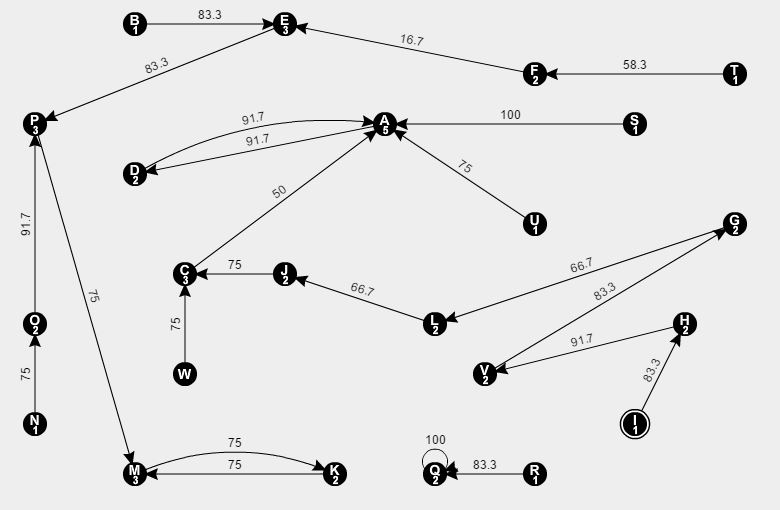
\includegraphics[totalheight=9cm, width=\textwidth]{Graph1}
\caption{Partial representation of trusted peers among survey respondents}
\end{figure}
\smallskip
\begin{figure}
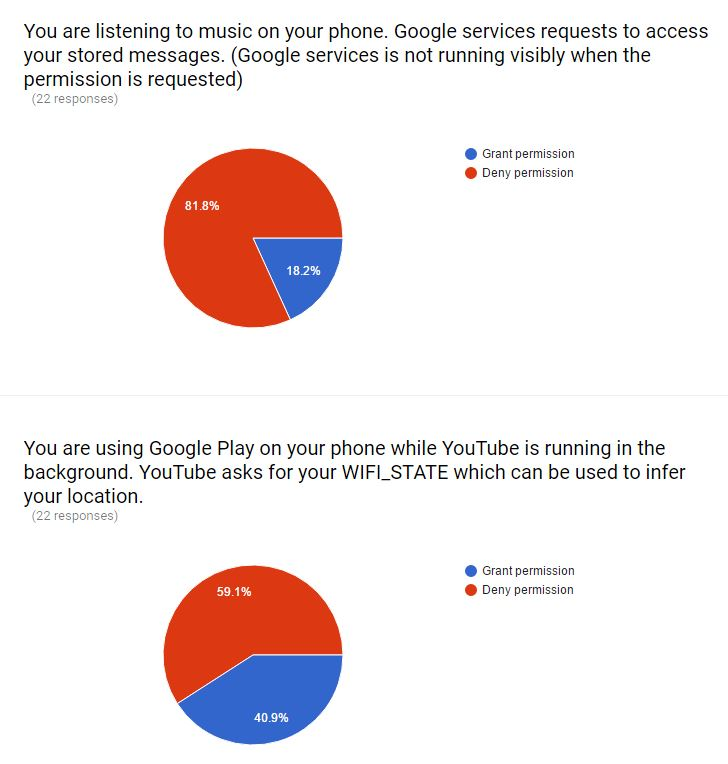
\includegraphics[ width=\textwidth]{Survey1}
\caption{Some responses from the survey}
\end{figure}

The partial data was represented using a graph(Figure 2.4). Participants were each assigned a letter of the alphabet. A directed edge from A to B denotes that A named B as a trusted peer, and the weight of an edge represents the percentage of similarity between the privacy choices of A and B. Each response was assigned a binary value( 1 for "grant permission" and 0 for "deny permission") and represented as a string, and the percentage of similarity was calculated using a Python string matching script. The weight assigned to each edge is represented as a percentage for ease of understanding. For example the edge from B->E denotes that B named E as a trusted peer, and B's privacy preferences match those of E 83.3\% of the time. Nodes with a higher indegree are people who are more "trusted" by their peers. Since each participant was asked to name \textit{one} "peer" all nodes have an outdegree of 1. 
\smallskip

The completed graph can be used as a measure to evaluate the difference in expectations and reality in terms of "trust transitivity" among the target group. Apart from the trust rating between E and F (16.7\%) all other responses show trust similarity among peers of 50\% or more. The average matching percentage is \textbf{75.72\%}. Since trust is subjective, it can be argued that the results are not conclusive in terms of similarity as even "peers" with a 100\% similarity may choose different privacy options depending on the context in which they occur. However the current permission model does not offer any reassurance that the permission decisions of users do not lead to privacy violations, as the context in which a granted permission is requested and utilized is not fully explained. Research\cite{wijesekera2015android} conducted to determine the similarity between user expectations when granting a permission and privacy violations which occur has shown that in versions before Marshmallow, user expectations are met only 25\% of the time, while there is an improvement to 80\% in newer versions of Android. However only 15.2\% of users have upgraded to devices with Android versions newer than Marshmallow\cite{androdashboard}. Compared to the success rate of the current install time model(25\%) the result shown from our model of 75\% is a 300\% improvement on the previous system(see table 2.1). 
\smallskip

\begin{table}[]
\centering
\begin{tabular}{|l|l|ll}
\cline{1-2}
                        & \textbf{Success Rate} &  &  \\ \cline{1-2}
\textbf{Ask-On-Install} & 25\%                  &  &  \\ \cline{1-2}
\textbf{Marshmallow}    & 80\%                  &  &  \\ \cline{1-2}
\textbf{Our approach}   & 75.72\%               &  &  \\ \cline{1-2}
\end{tabular}
\caption{Comparison of Partial Results}
\label{comp-results}
\end{table}


User habituation due to increased user involvement in privacy decision making is a key issue in Android versions newer than Marshmallow as well. Therefore even though Marshmallow has 80\% success rate it still requires extensive user involvement. However our approach significantly reduces the user habituation by letting the user adopt privacy preferences of someone they trust. In later stages of the research we hope to quantify the actual level of user involvement as well. There are additional factors to be considered such as the feasibility of adapting permission requests in every context, and applicability according to device versions. Our user group consisted of UCSC students who are relatively well-informed about privacy violations. Further analysis is required before proceeding with the proposed modifications to PlayStore apk which will enable users to choose to adopt privacy settings of more experienced peers and make more informed decisions about permission requests, and enable us to log actual user involvement and decrease in problems caused due to habituation. 






